\scanpage{72}
\mspage{71}

Je pense qu'on \unsure{arrive|aura} à un tel formalisme sans hyp. sur $I$ (genre ``tronçon ordonné'') à condition de tenir compte de la possibilité qu'il y ait des $1$-strates
\[
X=[a,b]\quad(a<b)
\]
réduites à $\{a,b\}$ (quand $]a,b[=\varnothing$). Dans ce cas, il serait déraisonnable de définir $\operatorname{supp}X=[a,b]$ \unsure{ce qui donne} $=\deleted{\unsure{\{a,b\}}}\operatorname{supp}\partial X$. Mais on doit pouvoir définir une notion de support, \unsure{p. associé} à une partie tot. ordonnée quelconque $\Delta$ de $I$ (\unsure{éventuellement}, $\Delta=\bigcup_\alpha\partial X_\alpha$)
\[
a_1<a_2\ \cdots\ <a_n
\]
comme étant \deleted{\unsure{tous les}} les éléments de l'algèbre de Boole sur l'ens des ``points''
\[
\{a_1\},[a_1,a_2],\{a_2\},[a_2,a_3],\ldots,\{a_n\}
\]

\deleted{Toute famille}\inserted{Pour} $\unsure{\mathscr{X}|\mathcal{X}}\subset M$, $\mathscr{X}=\{X_\alpha\}$, \uline{subordonnée} à $\Delta$ i.e. telle que $\partial X_\alpha\subset\Delta\quad\forall\alpha$, on définit $\operatorname{supp}\mathscr{X}$ comme partie de cet ens (partie fermée, en fait, qui est un ens ordonné de façon évidente\unsure{\}|)}, \unsure{sous|suivant} l'inclusion des \inserted{\unsure{vraies}} parties de $I$), et on définit de même le support d'une différence virtuelle $X\setminus Y$ pour $Y\ll X$, ou $F\setminus G$ pour $F\unsure{\ll|\leq}G$, $F,G$ figures dans la \deleted{\illegible{1}} partie $\leq$-fermée de $\unsure{\mathcal{F}|\mathscr{F}}$ engendrée par $\mathscr{X}$.

Mais ça signifie finalement que pour tte figure dans \unsure{une|un} chaîne, i.e.
\figure{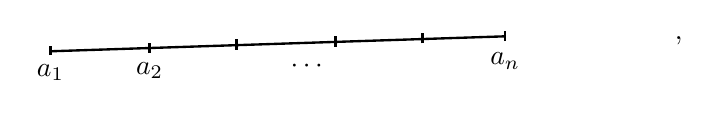
\begin{tikzpicture}[x=1.05cm,y=1cm,line width=0.85pt]
\draw (0,0)--(5.5,0.19);
\draw (0,-0.05)--(0,0.07) (1.2,-0.02)--(1.2,0.11) (2.25,0.02)--(2.25,0.15) (3.45,0.06)--(3.45,0.19) (4.5,0.1)--(4.5,0.23) (5.5,0.13)--(5.5,0.26);
\node[below] at (0,-0.04) {$a_1$};
\node[below] at (1.2,-0.01) {$a_2$};
\node[below] at (3.1,0.02) {$\cdots$};
\node[below] at (5.5,0.11) {$a_n$};
\node at (7.6,0.13) {,};
\end{tikzpicture}}
